\section{Lexer and Parser}
\label{lab06:parser}

As described above, lexer and parser are components of analyzer. Their task is to parse source code and provide statements for further processing.

\subsection{Overview}

For parser to be fully initialized, it needs several objects (see \cref{fig06:pars_lex}):
\begin{itemize}
	\item \emph{Input source} -- reads characters from the stream. Required by lexer.
	\item \emph{Lexer} -- creates tokens. Required by token stream.
	\item \emph{Token stream} -- buffers tokens. Required by parser.
	\item \emph{Parser} -- create statements with grammar rules.
\end{itemize}

This architecture, was employed with tool ANLTR 4 \footnote{\url{https://www.antlr.org}}. Each of the components is modified to comfort the language needs.

\begin{figure}
	\centering
	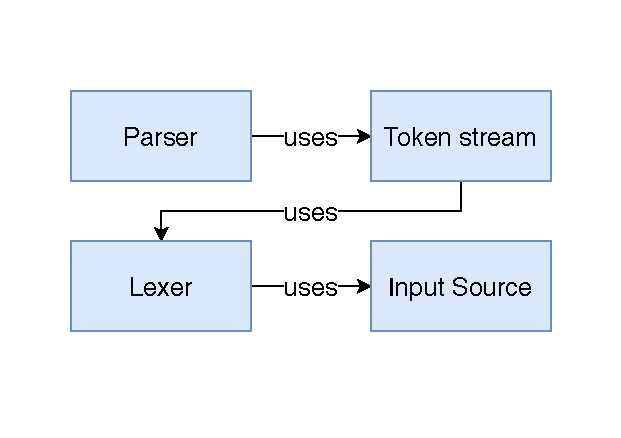
\includegraphics[width=\textwidth/2]{img/parser_lexer_arch}
	\caption{The composition of parser and lexer components.}
	\label{fig06:pars_lex}
\end{figure}

\subsection{Lexer}

Lexer's task is to read source string with help of input source object and break it into tokens --- small pieces of text with special meaning. 

The main features of lexer are:
\begin{enumerate}
	\item Checking whether all characters are valid in the HLASM source.
	\item Jumping in the source file backward and forward.
\end{enumerate}

The first feature .... ask Peter

The second feature is important for correct processing of AGO and AIF instructions. Because of this requirement, it is not possible to use any standard lexing tool. Therefore, the lexer had to be implemented from scratch.

\subsubsection{Token}

Contains location in the source. ... ask Peter


\subsection{Parser}

Parser component takes the lexer produced tokens from token stream and recognizes HLASM statements. To accomplish this, a parser generator tool ANTLR 4 \footnote{\url{https://www.antlr.org}} is used.

\subsubsection{ANTLR overview}

The input to ANTLR is a grammar written in antlr-specific language that specifies the syntax of HLASM language. The framework takes grammar and generates source code (in C++) for a recognizer, which is able to tell whether input source code is valid or not. Moreover, it is possible to assign a piece of code that executes every time a grammar rule is matched by the recognizer to further process the matched piece of code and produce helper structures (statements).

The parser inherits from the recognizer to provide further operations.

\subsubsection{Parser workflow}

Parser (in code reference as \TT{parser\_impl}) implements opencode statement provider interface. This means that, according to the statement passing in \cref{lab06:proc_stat}, parser needs to:
\begin{enumerate}
	\item Retrieve statement instruction field.
	\item Wait for the retrieval of the operand format by statement processor.
	\item Retrieve rest of the statement with respect to the passed format.
\end{enumerate} 

This has several consequences as grammar has to be prepared for that.
